\chapter{Definizione e alimentazione Data Mart}

\section{Progettazione Logica}

A partire dal DFM di figura~\ref{fig:dfm} è stato realizzato lo schema
logico del data warehouse rappresentato in figura~\ref{fig:logic}.
La scelta è stata quella di utilizzare il modello \textit{ROLAP} e di
implementare tale schema utilizzando il DBMS MySQL.
Lo schema utilizzato è quello a \textit{stella} al quale sono state applicate
delle variazioni al fine di eliminare alcune ridondanze e rendere più efficiente
in termini di spazio occupato le tabelle relative alle diverse dimensioni.
Si sceglie di mantenere i dati all'interno dei data mart per un orizzonte
temporale variabile tra i due e i 5 anni dalla data del loro inserimento.

La tabella \textit{vehicle\_use} costituisce il fatto e ha per attributi:
\begin{itemize}
\item le dimensioni \textit{start\_time}, \textit{end\_time}, \textit{city} e
\textit{vehicle\_type} che costituiscono insieme la chiave primaria della
tabella e sono ognuna chiave di una tabella in relazione con quella in oggetto;
\item le misure \textit{uses} e \textit{travelled\_distance};
\item \textit{weather\_id} e \textit{strike\_id} chiavi rispettivamente per
le tabelle \textit{weather} e \textit{strike}, attributi dimensionali della
dimensione \textit{city} all'interno del DFM sono stati inseriti all'interno
della tabella del fatto in qualità di attributi al fine di permettere in
fase di interrogazione di poter risalire più agevolmente agli stessi.
\end{itemize}

Per la tabella \textit{weather} è stata aggiunta una chiave surrogata che ha
permesso l'introduzione della relazione con la tabella del fatto, è stata
mantenuta la relazione con la tabella \textit{city} mediante la chiave
\textit{city\_id} e sono state eliminate le relazioni con la tabella
\textit{date} presenti nel DFM. Quest'ultima modifica ha permesso di
porre un vincolo di \java{UNIQUE} sulla tupla formata dagli attributi
\textit{wind\_level}, \textit{temperature\_level} e \textit{rain\_level}
evitando quindi di memorizzare più volte la stessa rilevazione per date
differenti.

La tabella \textit{date} ha come chiave primaria un attributo di tipo
\java{DATETIME} e riporta una serie di attributi ricavati dalla data utilizzata
come chiave quali \textit{day}, \textit{month}, \textit{year} e
\textit{weekday}.
si è scelto di creare tale tabella al fine di agevolare le interrogazioni, che
necessitano di selezionare una fascia oraria e/o uno o più giorni della
settimana, evitando di dover ricorrere all'uso di particolari funzioni del DBMS.

La tabella \textit{strike} aggiunge un attributo \textit{id}, chiave surrogata 
utile alla relazione con la tabella \textit{vehicle\_use}.

La tabella \textit{city} rimane pressoché invariata rispetto alla controparte
\textit{cities} appartenente allo schema riconciliato.

Si noti inoltre la presenza della tabella \textit{etl\_execution\_run} il cui
utilizzo è ristretto al processo di ETL descritto al paragrafo seguente.

\begin{figure}[H]                                                                                                                                                            
\centering                                                                                                                                                                   
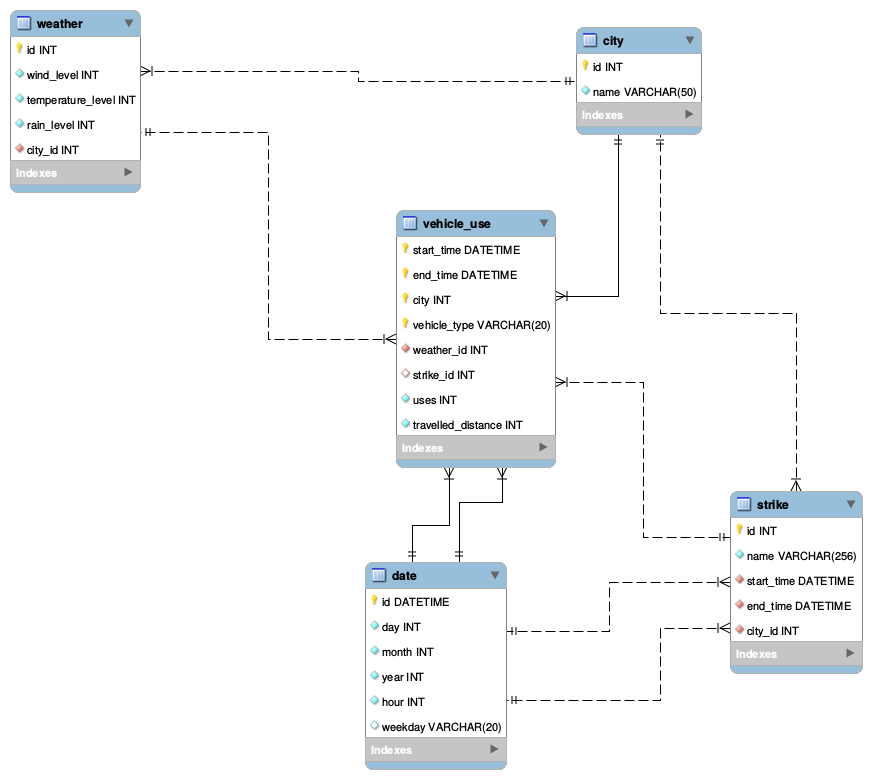
\includegraphics[width=\textwidth]{diagrams/logic}                                                                                                                                   
\caption{DFM Vehicle use}                                                                                                                                            
\label{fig:logic}                                                                                                                                                           
\end{figure}

\section{ETL da ODS a Data Mart}

E' necessario applicare un processo di ETL al fine di popolare le tabelle del
data mart definito al paragrafo precedente a partire dallo schema riconciliato
di figura~\ref{fig:riconciliato_er}. Tale processo, similmente a quello definito
per il popolamento dell'ODS a partire dai database delle singole sorgenti
operazionali, è di tipo \textit{incremental delayed}; non essendo i dati
precedentemente memorizzati all'interno del data mart soggetti ad aggiornamento,
la procedura consiste nell'aggiunta dei nuovi record relativi alle profilazioni
delle sorgenti Helbiz e Torinometeo e nell'aggiornamento sugli scioperi
intervenuti a due giorni dalla data in cui avviene l'aggiornamento.

La procedura prevede che il popolamento delle tabelle relative alle dimensioni
ed ai relativi attributi avvenga prima del popolamento della tabella relativa
al fatto al fine di non violare i vincoli di integrità referenziale definiti.

La seguente procedura, implementata in uno script sql, è lanciata da un job di
sistema ogni notte dopo la mezzanotte e fa seguito alla procedura di ETL
da sorgenti a ODS definita al paragrafo~\ref{sec:etl_sorgenti_ODS}.

\subsection{Popolamento tabelle dimensioni}

Mediante una query sulla tabella \textit{etl\_execution\_run} del data mart
viene ottenuta la data dell'ultima esecuzione del processo in oggetto e
memorizzata in una variabile. Segue nell'ordine il popolamento delle tabelle:
\begin{itemize}
\item \textit{city:} a partire dalla tabella \textit{cities} dell'ODS vengono
estratti i nomi delle città per le quali il valore della colonna
\textit{insert\_time} di tale tabella risultino essere successivi a quelli 
della data in memoria; ad ognuno dei record inseriti è associato un id
numerico incrementale che costituisce la chiave surrogata;
\item \textit{date:} a partire dalla tabella \textit{vehicle\_hourly\_profilings}
vengono selezionati i record per i quali l'attributo
\textit{start\_profiling\_time} risulta essere superiore alla data di ultimo
popolamento in memoria; a partire dai valori della colonna
\textit{start\_profiling\_time} vengono ottenuti per mezzo di funzioni del DBMS
i valori relativi a giorno, mese, anno e giorno della settimana i quali
corrisponderanno rispettivamente agli attributi \textit{day}, \textit{month},
\textit{year} e \textit{weekday} del relativo record da inserirsi nella tabella
in oggetto; l'attributo di origine costituirà invece la chiave primaria;
\item \textit{strike:} vengono selezionati i record della tabella \textit{strikes}
dell'ODS aventi un valore \textit{start\_time} maggiore o eguale a quello della
data in memoria; all'interno della stessa query, viene eseguita una JOIN con la
tabella \textit{cities} dell'ODS e un'altra JOIN con la tabella \textit{city}
del data mart al fine di ottenere la chiave surrogata relativa alla città
associata all'interno dell'ODS;
\item \textit{weather:} vengono selezionati i record della tabella
\textit{weather\_hourly\_profilings} aventi per l'attributo
\textit{start\_profiling\_time} valore successivo a quello della data in memoria;
come per il popolamento della tabella al punto precedente, nella stessa query,
viene effettuata una JOIN con la tabella \textit{cities} dell'ODS ed una con la
tabella \textit{city} al fine di ottenere la chiave surrogata relativa alla città
associata all'interno dell'ODS.
\end{itemize}

\subsection{Popolamento tabella fatto}

Viene eseguita una query sulla tabella \textit{vehicles\_hourly\_profilings}
dell'ODS e vengono selezionati i record per i quali l'attributo
\textit{start\_profiling\_time} risulta essere antecedente alla data di ultimo
popolamento presente in memoria. Per ottenere la chiave surrogata \textit{city\_id}
viene effettuata una JOIN con la tabella \textit{city} ed una con la tabella
\textit{cities} dell'ODS. La stessa cosa avviene per la chiave surrogata
\textit{weather\_id} che viene recuperata mediante una JOIN con la tabella
\textit{weather} e con la tabella \textit{weather\_hourly\_profilings}.
Per quanto riguarda la chiave \textit{weather\_id} essa è ottenuta per mezzo
dell'operazione di LEFT JOIN con la tabella \textit{weather} specificando
come condizione che gli attributi \textit{start\_profiling\_time} e ì
\textit{end\_profiling\_time} della tabella \textit{vehicles\_hourly\_profilings}
siano contenuti nell'intervallo definito dagli attributi \textit{start\_time} e
\textit{end\_time} della tabella \textit{strike} dell'ODS. Infatti, come anticipato
alla descrizione dello schema logico del data mart, mentre per ogni record della
tabella del fatto corrisponde un record della tabella \textit{weather} ciò non
vale per la tabella \textit{strike} dato che non ad ogni giorno del periodo
temporale analizzato è associato uno sciopero.

La procedura di ETL termina con l'inserimento della data di esecuzione nella
tabella \textit{etl\_execution\_run}.
